% Options for packages loaded elsewhere
\PassOptionsToPackage{unicode}{hyperref}
\PassOptionsToPackage{hyphens}{url}
\PassOptionsToPackage{dvipsnames,svgnames,x11names}{xcolor}
%
\documentclass[
  letterpaper,
  DIV=11,
  numbers=noendperiod]{scrartcl}

\usepackage{amsmath,amssymb}
\usepackage{iftex}
\ifPDFTeX
  \usepackage[T1]{fontenc}
  \usepackage[utf8]{inputenc}
  \usepackage{textcomp} % provide euro and other symbols
\else % if luatex or xetex
  \usepackage{unicode-math}
  \defaultfontfeatures{Scale=MatchLowercase}
  \defaultfontfeatures[\rmfamily]{Ligatures=TeX,Scale=1}
\fi
\usepackage{lmodern}
\ifPDFTeX\else  
    % xetex/luatex font selection
\fi
% Use upquote if available, for straight quotes in verbatim environments
\IfFileExists{upquote.sty}{\usepackage{upquote}}{}
\IfFileExists{microtype.sty}{% use microtype if available
  \usepackage[]{microtype}
  \UseMicrotypeSet[protrusion]{basicmath} % disable protrusion for tt fonts
}{}
\makeatletter
\@ifundefined{KOMAClassName}{% if non-KOMA class
  \IfFileExists{parskip.sty}{%
    \usepackage{parskip}
  }{% else
    \setlength{\parindent}{0pt}
    \setlength{\parskip}{6pt plus 2pt minus 1pt}}
}{% if KOMA class
  \KOMAoptions{parskip=half}}
\makeatother
\usepackage{xcolor}
\setlength{\emergencystretch}{3em} % prevent overfull lines
\setcounter{secnumdepth}{-\maxdimen} % remove section numbering
% Make \paragraph and \subparagraph free-standing
\makeatletter
\ifx\paragraph\undefined\else
  \let\oldparagraph\paragraph
  \renewcommand{\paragraph}{
    \@ifstar
      \xxxParagraphStar
      \xxxParagraphNoStar
  }
  \newcommand{\xxxParagraphStar}[1]{\oldparagraph*{#1}\mbox{}}
  \newcommand{\xxxParagraphNoStar}[1]{\oldparagraph{#1}\mbox{}}
\fi
\ifx\subparagraph\undefined\else
  \let\oldsubparagraph\subparagraph
  \renewcommand{\subparagraph}{
    \@ifstar
      \xxxSubParagraphStar
      \xxxSubParagraphNoStar
  }
  \newcommand{\xxxSubParagraphStar}[1]{\oldsubparagraph*{#1}\mbox{}}
  \newcommand{\xxxSubParagraphNoStar}[1]{\oldsubparagraph{#1}\mbox{}}
\fi
\makeatother

\usepackage{color}
\usepackage{fancyvrb}
\newcommand{\VerbBar}{|}
\newcommand{\VERB}{\Verb[commandchars=\\\{\}]}
\DefineVerbatimEnvironment{Highlighting}{Verbatim}{commandchars=\\\{\}}
% Add ',fontsize=\small' for more characters per line
\usepackage{framed}
\definecolor{shadecolor}{RGB}{241,243,245}
\newenvironment{Shaded}{\begin{snugshade}}{\end{snugshade}}
\newcommand{\AlertTok}[1]{\textcolor[rgb]{0.68,0.00,0.00}{#1}}
\newcommand{\AnnotationTok}[1]{\textcolor[rgb]{0.37,0.37,0.37}{#1}}
\newcommand{\AttributeTok}[1]{\textcolor[rgb]{0.40,0.45,0.13}{#1}}
\newcommand{\BaseNTok}[1]{\textcolor[rgb]{0.68,0.00,0.00}{#1}}
\newcommand{\BuiltInTok}[1]{\textcolor[rgb]{0.00,0.23,0.31}{#1}}
\newcommand{\CharTok}[1]{\textcolor[rgb]{0.13,0.47,0.30}{#1}}
\newcommand{\CommentTok}[1]{\textcolor[rgb]{0.37,0.37,0.37}{#1}}
\newcommand{\CommentVarTok}[1]{\textcolor[rgb]{0.37,0.37,0.37}{\textit{#1}}}
\newcommand{\ConstantTok}[1]{\textcolor[rgb]{0.56,0.35,0.01}{#1}}
\newcommand{\ControlFlowTok}[1]{\textcolor[rgb]{0.00,0.23,0.31}{\textbf{#1}}}
\newcommand{\DataTypeTok}[1]{\textcolor[rgb]{0.68,0.00,0.00}{#1}}
\newcommand{\DecValTok}[1]{\textcolor[rgb]{0.68,0.00,0.00}{#1}}
\newcommand{\DocumentationTok}[1]{\textcolor[rgb]{0.37,0.37,0.37}{\textit{#1}}}
\newcommand{\ErrorTok}[1]{\textcolor[rgb]{0.68,0.00,0.00}{#1}}
\newcommand{\ExtensionTok}[1]{\textcolor[rgb]{0.00,0.23,0.31}{#1}}
\newcommand{\FloatTok}[1]{\textcolor[rgb]{0.68,0.00,0.00}{#1}}
\newcommand{\FunctionTok}[1]{\textcolor[rgb]{0.28,0.35,0.67}{#1}}
\newcommand{\ImportTok}[1]{\textcolor[rgb]{0.00,0.46,0.62}{#1}}
\newcommand{\InformationTok}[1]{\textcolor[rgb]{0.37,0.37,0.37}{#1}}
\newcommand{\KeywordTok}[1]{\textcolor[rgb]{0.00,0.23,0.31}{\textbf{#1}}}
\newcommand{\NormalTok}[1]{\textcolor[rgb]{0.00,0.23,0.31}{#1}}
\newcommand{\OperatorTok}[1]{\textcolor[rgb]{0.37,0.37,0.37}{#1}}
\newcommand{\OtherTok}[1]{\textcolor[rgb]{0.00,0.23,0.31}{#1}}
\newcommand{\PreprocessorTok}[1]{\textcolor[rgb]{0.68,0.00,0.00}{#1}}
\newcommand{\RegionMarkerTok}[1]{\textcolor[rgb]{0.00,0.23,0.31}{#1}}
\newcommand{\SpecialCharTok}[1]{\textcolor[rgb]{0.37,0.37,0.37}{#1}}
\newcommand{\SpecialStringTok}[1]{\textcolor[rgb]{0.13,0.47,0.30}{#1}}
\newcommand{\StringTok}[1]{\textcolor[rgb]{0.13,0.47,0.30}{#1}}
\newcommand{\VariableTok}[1]{\textcolor[rgb]{0.07,0.07,0.07}{#1}}
\newcommand{\VerbatimStringTok}[1]{\textcolor[rgb]{0.13,0.47,0.30}{#1}}
\newcommand{\WarningTok}[1]{\textcolor[rgb]{0.37,0.37,0.37}{\textit{#1}}}

\providecommand{\tightlist}{%
  \setlength{\itemsep}{0pt}\setlength{\parskip}{0pt}}\usepackage{longtable,booktabs,array}
\usepackage{calc} % for calculating minipage widths
% Correct order of tables after \paragraph or \subparagraph
\usepackage{etoolbox}
\makeatletter
\patchcmd\longtable{\par}{\if@noskipsec\mbox{}\fi\par}{}{}
\makeatother
% Allow footnotes in longtable head/foot
\IfFileExists{footnotehyper.sty}{\usepackage{footnotehyper}}{\usepackage{footnote}}
\makesavenoteenv{longtable}
\usepackage{graphicx}
\makeatletter
\def\maxwidth{\ifdim\Gin@nat@width>\linewidth\linewidth\else\Gin@nat@width\fi}
\def\maxheight{\ifdim\Gin@nat@height>\textheight\textheight\else\Gin@nat@height\fi}
\makeatother
% Scale images if necessary, so that they will not overflow the page
% margins by default, and it is still possible to overwrite the defaults
% using explicit options in \includegraphics[width, height, ...]{}
\setkeys{Gin}{width=\maxwidth,height=\maxheight,keepaspectratio}
% Set default figure placement to htbp
\makeatletter
\def\fps@figure{htbp}
\makeatother

\KOMAoption{captions}{tableheading}
\makeatletter
\@ifpackageloaded{caption}{}{\usepackage{caption}}
\AtBeginDocument{%
\ifdefined\contentsname
  \renewcommand*\contentsname{Table of contents}
\else
  \newcommand\contentsname{Table of contents}
\fi
\ifdefined\listfigurename
  \renewcommand*\listfigurename{List of Figures}
\else
  \newcommand\listfigurename{List of Figures}
\fi
\ifdefined\listtablename
  \renewcommand*\listtablename{List of Tables}
\else
  \newcommand\listtablename{List of Tables}
\fi
\ifdefined\figurename
  \renewcommand*\figurename{Figure}
\else
  \newcommand\figurename{Figure}
\fi
\ifdefined\tablename
  \renewcommand*\tablename{Table}
\else
  \newcommand\tablename{Table}
\fi
}
\@ifpackageloaded{float}{}{\usepackage{float}}
\floatstyle{ruled}
\@ifundefined{c@chapter}{\newfloat{codelisting}{h}{lop}}{\newfloat{codelisting}{h}{lop}[chapter]}
\floatname{codelisting}{Listing}
\newcommand*\listoflistings{\listof{codelisting}{List of Listings}}
\makeatother
\makeatletter
\makeatother
\makeatletter
\@ifpackageloaded{caption}{}{\usepackage{caption}}
\@ifpackageloaded{subcaption}{}{\usepackage{subcaption}}
\makeatother

\ifLuaTeX
  \usepackage{selnolig}  % disable illegal ligatures
\fi
\usepackage{bookmark}

\IfFileExists{xurl.sty}{\usepackage{xurl}}{} % add URL line breaks if available
\urlstyle{same} % disable monospaced font for URLs
\hypersetup{
  pdftitle={Adverse Event EDA for \{params\$drug\}},
  pdfauthor={Shohn Godboldt},
  colorlinks=true,
  linkcolor={blue},
  filecolor={Maroon},
  citecolor={Blue},
  urlcolor={Blue},
  pdfcreator={LaTeX via pandoc}}


\title{Adverse Event EDA for \{params\$drug\}}
\author{Shohn Godboldt}
\date{}

\begin{document}
\maketitle


\subsection{1. Objective \& Business
Framing}\label{objective-business-framing}

\textbf{Goal.} Use a public healthcare API to practice advisor-style
EDA: quantify \textbf{adverse events} for a given drug, identify
\textbf{top reactions}, \textbf{age/sex patterns}, \textbf{serious
outcomes}, and \textbf{time trends}.\\
\textbf{Why it matters.} Payers and health plans track safety signals to
inform care management, member outreach, and provider education.

\begin{center}\rule{0.5\linewidth}{0.5pt}\end{center}

\subsection{2. Data Source \& Pull (openFDA Drug Event
API)}\label{data-source-pull-openfda-drug-event-api}

We query: \texttt{https://api.fda.gov/drug/event.json} (no key
required). We'll filter by \textbf{receivedate} and \textbf{drug name}.

\begin{Shaded}
\begin{Highlighting}[]
\NormalTok{fetch\_openfda\_page }\OtherTok{\textless{}{-}} \ControlFlowTok{function}\NormalTok{(search, }\AttributeTok{skip =} \DecValTok{0}\NormalTok{, }\AttributeTok{limit =} \DecValTok{1000}\NormalTok{) \{}
\NormalTok{  base }\OtherTok{\textless{}{-}} \StringTok{"https://api.fda.gov/drug/event.json"}
\NormalTok{  url  }\OtherTok{\textless{}{-}} \FunctionTok{glue}\NormalTok{(}\StringTok{"\{base\}?search=\{URLencode(search)\}\&limit=\{limit\}\&skip=\{skip\}"}\NormalTok{)}
  \FunctionTok{tryCatch}\NormalTok{(jsonlite}\SpecialCharTok{::}\FunctionTok{fromJSON}\NormalTok{(url), }\AttributeTok{error =} \ControlFlowTok{function}\NormalTok{(e) }\ConstantTok{NULL}\NormalTok{)}
\NormalTok{\}}

\CommentTok{\# Robust total estimator (fast probe, then fallback to count endpoint)}
\NormalTok{count\_openfda }\OtherTok{\textless{}{-}} \ControlFlowTok{function}\NormalTok{(search) \{}
\NormalTok{  base }\OtherTok{\textless{}{-}} \StringTok{"https://api.fda.gov/drug/event.json"}
\NormalTok{  probe\_url }\OtherTok{\textless{}{-}} \FunctionTok{glue}\NormalTok{(}\StringTok{"\{base\}?search=\{URLencode(search)\}\&limit=1"}\NormalTok{)}
\NormalTok{  res }\OtherTok{\textless{}{-}} \FunctionTok{tryCatch}\NormalTok{(jsonlite}\SpecialCharTok{::}\FunctionTok{fromJSON}\NormalTok{(probe\_url), }\AttributeTok{error =} \ControlFlowTok{function}\NormalTok{(e) }\ConstantTok{NULL}\NormalTok{)}
\NormalTok{  tot }\OtherTok{\textless{}{-}} \FunctionTok{suppressWarnings}\NormalTok{(}\FunctionTok{as.integer}\NormalTok{(}\FunctionTok{tryCatch}\NormalTok{(res}\SpecialCharTok{$}\NormalTok{meta}\SpecialCharTok{$}\NormalTok{results}\SpecialCharTok{$}\NormalTok{total, }\AttributeTok{error =} \ControlFlowTok{function}\NormalTok{(e) }\ConstantTok{NA\_integer\_}\NormalTok{)))}
  \ControlFlowTok{if}\NormalTok{ (}\SpecialCharTok{!}\FunctionTok{is.na}\NormalTok{(tot)) }\FunctionTok{return}\NormalTok{(tot)}

\NormalTok{  url2 }\OtherTok{\textless{}{-}} \FunctionTok{glue}\NormalTok{(}\StringTok{"\{base\}?search=\{URLencode(search)\}\&count=receivedate"}\NormalTok{)}
\NormalTok{  res2 }\OtherTok{\textless{}{-}} \FunctionTok{tryCatch}\NormalTok{(jsonlite}\SpecialCharTok{::}\FunctionTok{fromJSON}\NormalTok{(url2), }\AttributeTok{error =} \ControlFlowTok{function}\NormalTok{(e) }\ConstantTok{NULL}\NormalTok{)}
  \ControlFlowTok{if}\NormalTok{ (}\FunctionTok{is.null}\NormalTok{(res2) }\SpecialCharTok{||} \FunctionTok{is.null}\NormalTok{(res2}\SpecialCharTok{$}\NormalTok{results)) }\FunctionTok{return}\NormalTok{(}\DecValTok{0}\NormalTok{L)}
  \ControlFlowTok{if}\NormalTok{ (}\FunctionTok{is.data.frame}\NormalTok{(res2}\SpecialCharTok{$}\NormalTok{results) }\SpecialCharTok{\&\&} \StringTok{"count"} \SpecialCharTok{\%in\%} \FunctionTok{names}\NormalTok{(res2}\SpecialCharTok{$}\NormalTok{results)) \{}
    \FunctionTok{return}\NormalTok{(}\FunctionTok{sum}\NormalTok{(res2}\SpecialCharTok{$}\NormalTok{results}\SpecialCharTok{$}\NormalTok{count, }\AttributeTok{na.rm =} \ConstantTok{TRUE}\NormalTok{))}
\NormalTok{  \}}
  \DecValTok{0}\NormalTok{L}
\NormalTok{\}}

\StringTok{\textasciigrave{}}\AttributeTok{\%||\%}\StringTok{\textasciigrave{}} \OtherTok{\textless{}{-}} \ControlFlowTok{function}\NormalTok{(a,b) }\ControlFlowTok{if}\NormalTok{ (}\FunctionTok{is.null}\NormalTok{(a)) b }\ControlFlowTok{else}\NormalTok{ a}
\end{Highlighting}
\end{Shaded}

\begin{Shaded}
\begin{Highlighting}[]
\NormalTok{alias\_terms }\OtherTok{\textless{}{-}} \ControlFlowTok{function}\NormalTok{(drug\_in) \{}
\NormalTok{  d }\OtherTok{\textless{}{-}} \FunctionTok{tolower}\NormalTok{(}\FunctionTok{trimws}\NormalTok{(drug\_in))}
  \ControlFlowTok{if}\NormalTok{ (d }\SpecialCharTok{==} \StringTok{"semaglutide"}\NormalTok{) \{}
    \FunctionTok{c}\NormalTok{(}\StringTok{"semaglutide"}\NormalTok{,}\StringTok{"ozempic"}\NormalTok{,}\StringTok{"wegovy"}\NormalTok{,}\StringTok{"rybelsus"}\NormalTok{)}
\NormalTok{  \} }\ControlFlowTok{else} \ControlFlowTok{if}\NormalTok{ (d }\SpecialCharTok{==} \StringTok{"metformin"}\NormalTok{) \{}
    \FunctionTok{c}\NormalTok{(}\StringTok{"metformin"}\NormalTok{,}\StringTok{"glucophage"}\NormalTok{)}
\NormalTok{  \} }\ControlFlowTok{else} \ControlFlowTok{if}\NormalTok{ (d }\SpecialCharTok{==} \StringTok{"atorvastatin"}\NormalTok{) \{}
    \FunctionTok{c}\NormalTok{(}\StringTok{"atorvastatin"}\NormalTok{,}\StringTok{"lipitor"}\NormalTok{)}
\NormalTok{  \} }\ControlFlowTok{else} \ControlFlowTok{if}\NormalTok{ (d }\SpecialCharTok{==} \StringTok{"amoxicillin"}\NormalTok{) \{}
    \FunctionTok{c}\NormalTok{(}\StringTok{"amoxicillin"}\NormalTok{,}\StringTok{"amoxil"}\NormalTok{)}
\NormalTok{  \} }\ControlFlowTok{else}\NormalTok{ \{}
    \FunctionTok{c}\NormalTok{(d)}
\NormalTok{  \}}
\NormalTok{\}}
\end{Highlighting}
\end{Shaded}

\begin{Shaded}
\begin{Highlighting}[]
\CommentTok{\# {-}{-}{-}{-} Speed knobs (adjust as needed) {-}{-}{-}{-}}
\NormalTok{MAX\_PULL\_CAP }\OtherTok{\textless{}{-}} \DecValTok{2500}\NormalTok{L}
\NormalTok{PAGE\_LIMIT   }\OtherTok{\textless{}{-}} \DecValTok{500}\NormalTok{L}

\CommentTok{\# Build search with patient.drug.* and OR\textquotesingle{}ed generic/brand names}
\NormalTok{terms }\OtherTok{\textless{}{-}} \FunctionTok{alias\_terms}\NormalTok{(drug)}
\NormalTok{term\_clauses  }\OtherTok{\textless{}{-}} \FunctionTok{sprintf}\NormalTok{(}\StringTok{\textquotesingle{}patient.drug.medicinalproduct:"\%s"\textquotesingle{}}\NormalTok{, terms)}
\NormalTok{term\_clauses2 }\OtherTok{\textless{}{-}} \FunctionTok{c}\NormalTok{(}
  \FunctionTok{sprintf}\NormalTok{(}\StringTok{\textquotesingle{}patient.drug.openfda.generic\_name:"\%s"\textquotesingle{}}\NormalTok{, }\FunctionTok{toupper}\NormalTok{(terms)),}
  \FunctionTok{sprintf}\NormalTok{(}\StringTok{\textquotesingle{}patient.drug.openfda.brand\_name:"\%s"\textquotesingle{}}\NormalTok{,   }\FunctionTok{toupper}\NormalTok{(terms))}
\NormalTok{)}

\NormalTok{drug\_query }\OtherTok{\textless{}{-}} \FunctionTok{paste}\NormalTok{(}\FunctionTok{c}\NormalTok{(term\_clauses, term\_clauses2), }\AttributeTok{collapse =} \StringTok{"+OR+"}\NormalTok{)}
\NormalTok{q\_drug     }\OtherTok{\textless{}{-}} \FunctionTok{paste0}\NormalTok{(}\StringTok{"("}\NormalTok{, drug\_query, }\StringTok{")"}\NormalTok{)}
\NormalTok{q\_dates    }\OtherTok{\textless{}{-}} \FunctionTok{glue}\NormalTok{(}\StringTok{"receivedate:[\{format(start\_date, \textquotesingle{}\%Y\%m\%d\textquotesingle{})\}+TO+\{format(end\_date, \textquotesingle{}\%Y\%m\%d\textquotesingle{})\}]"}\NormalTok{)}

\CommentTok{\# Build single{-}string query (avoid vector/brace issues)}
\NormalTok{search }\OtherTok{\textless{}{-}} \FunctionTok{glue}\NormalTok{(}\StringTok{"\{q\_drug\}+AND+\{q\_dates\}"}\NormalTok{)}
\NormalTok{search }\OtherTok{\textless{}{-}} \FunctionTok{paste}\NormalTok{(search, }\AttributeTok{collapse =} \StringTok{" "}\NormalTok{)}

\CommentTok{\# Count; if zero, broaden dates and retry once}
\NormalTok{total\_est }\OtherTok{\textless{}{-}} \FunctionTok{count\_openfda}\NormalTok{(search)}
\ControlFlowTok{if}\NormalTok{ (total\_est }\SpecialCharTok{==} \DecValTok{0}\NormalTok{) \{}
\NormalTok{  start\_date }\OtherTok{\textless{}{-}} \FunctionTok{as.Date}\NormalTok{(}\StringTok{"2019{-}01{-}01"}\NormalTok{)}
\NormalTok{  q\_dates    }\OtherTok{\textless{}{-}} \FunctionTok{glue}\NormalTok{(}\StringTok{"receivedate:[\{format(start\_date, \textquotesingle{}\%Y\%m\%d\textquotesingle{})\}+TO+\{format(end\_date, \textquotesingle{}\%Y\%m\%d\textquotesingle{})\}]"}\NormalTok{)}
\NormalTok{  search     }\OtherTok{\textless{}{-}} \FunctionTok{glue}\NormalTok{(}\StringTok{"\{q\_drug\}+AND+\{q\_dates\}"}\NormalTok{)}
\NormalTok{  search     }\OtherTok{\textless{}{-}} \FunctionTok{paste}\NormalTok{(search, }\AttributeTok{collapse =} \StringTok{" "}\NormalTok{)}
\NormalTok{  total\_est  }\OtherTok{\textless{}{-}} \FunctionTok{count\_openfda}\NormalTok{(search)}
\NormalTok{\}}
\ControlFlowTok{if}\NormalTok{ (total\_est }\SpecialCharTok{==} \DecValTok{0}\NormalTok{) }\FunctionTok{stop}\NormalTok{(}\StringTok{"No records found after alias + broadened dates. Try another drug or dates."}\NormalTok{)}

\CommentTok{\# {-}{-}{-}{-} Caching {-}{-}{-}{-}}
\NormalTok{cache\_path }\OtherTok{\textless{}{-}} \FunctionTok{glue}\NormalTok{(}
  \StringTok{"data/raw\_\{drug\}\_\{format(start\_date, \textquotesingle{}\%Y\%m\%d\textquotesingle{})\}\_\{format(end\_date, \textquotesingle{}\%Y\%m\%d\textquotesingle{})\}\_\{MAX\_PULL\_CAP\}\_\{PAGE\_LIMIT\}.rds"}
\NormalTok{)}

\ControlFlowTok{if}\NormalTok{ (}\FunctionTok{file.exists}\NormalTok{(cache\_path)) \{}
\NormalTok{  all\_results }\OtherTok{\textless{}{-}} \FunctionTok{readRDS}\NormalTok{(cache\_path)}

\NormalTok{\} }\ControlFlowTok{else}\NormalTok{ \{}
\NormalTok{  max\_pull }\OtherTok{\textless{}{-}} \FunctionTok{min}\NormalTok{(}\FunctionTok{as.integer}\NormalTok{(total\_est), MAX\_PULL\_CAP)}
\NormalTok{  pages    }\OtherTok{\textless{}{-}} \FunctionTok{ceiling}\NormalTok{(max\_pull }\SpecialCharTok{/}\NormalTok{ PAGE\_LIMIT)}

\NormalTok{  pull\_event\_chunk }\OtherTok{\textless{}{-}} \ControlFlowTok{function}\NormalTok{(skip) \{}
\NormalTok{    base }\OtherTok{\textless{}{-}} \StringTok{"https://api.fda.gov/drug/event.json"}
\NormalTok{    url  }\OtherTok{\textless{}{-}} \FunctionTok{glue}\NormalTok{(}\StringTok{"\{base\}?search=\{URLencode(search)\}\&limit=\{PAGE\_LIMIT\}\&skip=\{skip\}"}\NormalTok{)}
\NormalTok{    json }\OtherTok{\textless{}{-}} \FunctionTok{tryCatch}\NormalTok{(jsonlite}\SpecialCharTok{::}\FunctionTok{fromJSON}\NormalTok{(url), }\AttributeTok{error =} \ControlFlowTok{function}\NormalTok{(e) }\ConstantTok{NULL}\NormalTok{)}
    \ControlFlowTok{if}\NormalTok{ (}\FunctionTok{is.null}\NormalTok{(json) }\SpecialCharTok{||} \FunctionTok{is.null}\NormalTok{(json}\SpecialCharTok{$}\NormalTok{results)) }\FunctionTok{return}\NormalTok{(}\ConstantTok{NULL}\NormalTok{)}
\NormalTok{    json}\SpecialCharTok{$}\NormalTok{results}
\NormalTok{  \}}

\NormalTok{  all\_results }\OtherTok{\textless{}{-}}\NormalTok{ purrr}\SpecialCharTok{::}\FunctionTok{map}\NormalTok{(}
      \FunctionTok{seq}\NormalTok{(}\DecValTok{0}\NormalTok{, }\AttributeTok{by =}\NormalTok{ PAGE\_LIMIT, }\AttributeTok{length.out =}\NormalTok{ pages),}
\NormalTok{      pull\_event\_chunk}
\NormalTok{    ) }\SpecialCharTok{|\textgreater{}}
\NormalTok{    purrr}\SpecialCharTok{::}\FunctionTok{compact}\NormalTok{() }\SpecialCharTok{|\textgreater{}}
\NormalTok{    dplyr}\SpecialCharTok{::}\FunctionTok{bind\_rows}\NormalTok{()}

  \FunctionTok{saveRDS}\NormalTok{(all\_results, cache\_path)}
\NormalTok{\}}
\end{Highlighting}
\end{Shaded}

\begin{center}\rule{0.5\linewidth}{0.5pt}\end{center}

\subsection{3. Normalization \& Tidy
Model}\label{normalization-tidy-model}

We unnest to one row per \textbf{(safety report × reaction)} with key
fields.

\begin{Shaded}
\begin{Highlighting}[]
\CommentTok{\# Convert API results to a tibble and keep the patient list{-}column}
\NormalTok{events\_raw }\OtherTok{\textless{}{-}}\NormalTok{ tibble}\SpecialCharTok{::}\FunctionTok{as\_tibble}\NormalTok{(all\_results)}

\CommentTok{\# some payloads have safetyreportid only; others may also have id}
\NormalTok{has\_id }\OtherTok{\textless{}{-}} \StringTok{"id"} \SpecialCharTok{\%in\%} \FunctionTok{names}\NormalTok{(events\_raw)}

\NormalTok{tidy\_events }\OtherTok{\textless{}{-}}\NormalTok{ events\_raw }\SpecialCharTok{\%\textgreater{}\%}
\NormalTok{  dplyr}\SpecialCharTok{::}\FunctionTok{transmute}\NormalTok{(}
    \AttributeTok{safetyreportid =} \ControlFlowTok{if}\NormalTok{ (has\_id) dplyr}\SpecialCharTok{::}\FunctionTok{coalesce}\NormalTok{(safetyreportid, id) }\ControlFlowTok{else}\NormalTok{ safetyreportid,}
    \AttributeTok{receivedate    =}\NormalTok{ lubridate}\SpecialCharTok{::}\FunctionTok{ymd}\NormalTok{(receivedate),}
    \AttributeTok{seriousness    =}\NormalTok{ dplyr}\SpecialCharTok{::}\FunctionTok{coalesce}\NormalTok{(}\FunctionTok{as.integer}\NormalTok{(serious), }\DecValTok{0}\NormalTok{L),}
    \AttributeTok{patient        =}\NormalTok{ patient}
\NormalTok{  )}

\CommentTok{\# {-}{-}{-}{-} robust helpers (handle NULL/atomic/weird shapes) {-}{-}{-}{-}}
\NormalTok{safe\_extract\_age }\OtherTok{\textless{}{-}} \ControlFlowTok{function}\NormalTok{(p) \{}
  \ControlFlowTok{if}\NormalTok{ (}\FunctionTok{is.null}\NormalTok{(p) }\SpecialCharTok{||} \FunctionTok{is.atomic}\NormalTok{(p) }\SpecialCharTok{||} \FunctionTok{length}\NormalTok{(p) }\SpecialCharTok{==} \DecValTok{0}\NormalTok{) }\FunctionTok{return}\NormalTok{(}\ConstantTok{NA\_real\_}\NormalTok{)}
  \ControlFlowTok{if}\NormalTok{ (}\FunctionTok{inherits}\NormalTok{(p, }\StringTok{"data.frame"}\NormalTok{)) p }\OtherTok{\textless{}{-}} \FunctionTok{as.list}\NormalTok{(p)}
\NormalTok{  ag   }\OtherTok{\textless{}{-}} \FunctionTok{tryCatch}\NormalTok{(p}\SpecialCharTok{$}\NormalTok{patientonsetage,     }\AttributeTok{error =} \ControlFlowTok{function}\NormalTok{(e) }\ConstantTok{NULL}\NormalTok{)}
\NormalTok{  unit }\OtherTok{\textless{}{-}} \FunctionTok{tryCatch}\NormalTok{(p}\SpecialCharTok{$}\NormalTok{patientonsetageunit, }\AttributeTok{error =} \ControlFlowTok{function}\NormalTok{(e) }\ConstantTok{NULL}\NormalTok{)}
  \ControlFlowTok{if}\NormalTok{ (}\FunctionTok{is.null}\NormalTok{(ag)) }\FunctionTok{return}\NormalTok{(}\ConstantTok{NA\_real\_}\NormalTok{)}
\NormalTok{  ag }\OtherTok{\textless{}{-}} \FunctionTok{suppressWarnings}\NormalTok{(}\FunctionTok{as.numeric}\NormalTok{(ag[}\DecValTok{1}\NormalTok{]))}
  \ControlFlowTok{if}\NormalTok{ (}\FunctionTok{is.na}\NormalTok{(ag)) }\FunctionTok{return}\NormalTok{(}\ConstantTok{NA\_real\_}\NormalTok{)}
  \ControlFlowTok{if}\NormalTok{ (}\FunctionTok{is.null}\NormalTok{(unit)) }\FunctionTok{return}\NormalTok{(ag)}
\NormalTok{  unit }\OtherTok{\textless{}{-}} \FunctionTok{suppressWarnings}\NormalTok{(}\FunctionTok{as.numeric}\NormalTok{(unit[}\DecValTok{1}\NormalTok{]))}
  \ControlFlowTok{if}\NormalTok{ (}\FunctionTok{is.na}\NormalTok{(unit)) }\FunctionTok{return}\NormalTok{(ag)}
  \ControlFlowTok{if}\NormalTok{ (unit }\SpecialCharTok{==} \DecValTok{801}\NormalTok{) }\FunctionTok{return}\NormalTok{(ag }\SpecialCharTok{*} \DecValTok{10}\NormalTok{)  }\CommentTok{\# decades → years}
  \ControlFlowTok{if}\NormalTok{ (unit }\SpecialCharTok{==} \DecValTok{1}\NormalTok{)   }\FunctionTok{return}\NormalTok{(ag)       }\CommentTok{\# years}
\NormalTok{  ag}
\NormalTok{\}}

\NormalTok{safe\_extract\_sex }\OtherTok{\textless{}{-}} \ControlFlowTok{function}\NormalTok{(p) \{}
  \ControlFlowTok{if}\NormalTok{ (}\FunctionTok{is.null}\NormalTok{(p) }\SpecialCharTok{||} \FunctionTok{is.atomic}\NormalTok{(p) }\SpecialCharTok{||} \FunctionTok{length}\NormalTok{(p) }\SpecialCharTok{==} \DecValTok{0}\NormalTok{) }\FunctionTok{return}\NormalTok{(}\ConstantTok{NA\_character\_}\NormalTok{)}
  \ControlFlowTok{if}\NormalTok{ (}\FunctionTok{inherits}\NormalTok{(p, }\StringTok{"data.frame"}\NormalTok{)) p }\OtherTok{\textless{}{-}} \FunctionTok{as.list}\NormalTok{(p)}
\NormalTok{  sx }\OtherTok{\textless{}{-}} \FunctionTok{suppressWarnings}\NormalTok{(}\FunctionTok{as.integer}\NormalTok{(}\FunctionTok{tryCatch}\NormalTok{(p}\SpecialCharTok{$}\NormalTok{patientsex, }\AttributeTok{error =} \ControlFlowTok{function}\NormalTok{(e) }\ConstantTok{NA\_integer\_}\NormalTok{)))}
\NormalTok{  dplyr}\SpecialCharTok{::}\FunctionTok{case\_when}\NormalTok{(}
    \FunctionTok{is.na}\NormalTok{(sx) }\SpecialCharTok{\textasciitilde{}} \ConstantTok{NA\_character\_}\NormalTok{,}
\NormalTok{    sx }\SpecialCharTok{==} \DecValTok{1}   \SpecialCharTok{\textasciitilde{}} \StringTok{"Male"}\NormalTok{,}
\NormalTok{    sx }\SpecialCharTok{==} \DecValTok{2}   \SpecialCharTok{\textasciitilde{}} \StringTok{"Female"}\NormalTok{,}
    \ConstantTok{TRUE}      \SpecialCharTok{\textasciitilde{}} \StringTok{"Unknown"}
\NormalTok{  )}
\NormalTok{\}}

\NormalTok{safe\_unwrap\_reactions }\OtherTok{\textless{}{-}} \ControlFlowTok{function}\NormalTok{(p) \{}
  \ControlFlowTok{if}\NormalTok{ (}\FunctionTok{is.null}\NormalTok{(p) }\SpecialCharTok{||} \FunctionTok{is.atomic}\NormalTok{(p) }\SpecialCharTok{||} \FunctionTok{length}\NormalTok{(p) }\SpecialCharTok{==} \DecValTok{0}\NormalTok{)}
    \FunctionTok{return}\NormalTok{(tibble}\SpecialCharTok{::}\FunctionTok{tibble}\NormalTok{(}\AttributeTok{reaction =} \ConstantTok{NA\_character\_}\NormalTok{))}
\NormalTok{  rx }\OtherTok{\textless{}{-}} \FunctionTok{tryCatch}\NormalTok{(p}\SpecialCharTok{$}\NormalTok{reaction, }\AttributeTok{error =} \ControlFlowTok{function}\NormalTok{(e) }\ConstantTok{NULL}\NormalTok{)}
  \ControlFlowTok{if}\NormalTok{ (}\FunctionTok{is.null}\NormalTok{(rx)) }\FunctionTok{return}\NormalTok{(tibble}\SpecialCharTok{::}\FunctionTok{tibble}\NormalTok{(}\AttributeTok{reaction =} \ConstantTok{NA\_character\_}\NormalTok{))}
\NormalTok{  tibble}\SpecialCharTok{::}\FunctionTok{tibble}\NormalTok{(}\AttributeTok{reaction =} \FunctionTok{tolower}\NormalTok{(rx}\SpecialCharTok{$}\NormalTok{reactionmeddrapt))}
\NormalTok{\}}

\NormalTok{safe\_unwrap\_drugnames }\OtherTok{\textless{}{-}} \ControlFlowTok{function}\NormalTok{(p) \{}
  \ControlFlowTok{if}\NormalTok{ (}\FunctionTok{is.null}\NormalTok{(p) }\SpecialCharTok{||} \FunctionTok{is.atomic}\NormalTok{(p) }\SpecialCharTok{||} \FunctionTok{length}\NormalTok{(p) }\SpecialCharTok{==} \DecValTok{0}\NormalTok{) }\FunctionTok{return}\NormalTok{(}\ConstantTok{NA\_character\_}\NormalTok{)}
\NormalTok{  dr }\OtherTok{\textless{}{-}} \FunctionTok{tryCatch}\NormalTok{(p}\SpecialCharTok{$}\NormalTok{drug, }\AttributeTok{error =} \ControlFlowTok{function}\NormalTok{(e) }\ConstantTok{NULL}\NormalTok{)}
  \ControlFlowTok{if}\NormalTok{ (}\FunctionTok{is.null}\NormalTok{(dr)) }\FunctionTok{return}\NormalTok{(}\ConstantTok{NA\_character\_}\NormalTok{)}
\NormalTok{  prods }\OtherTok{\textless{}{-}} \FunctionTok{tolower}\NormalTok{(dr}\SpecialCharTok{$}\NormalTok{medicinalproduct)}
  \FunctionTok{paste}\NormalTok{(}\FunctionTok{unique}\NormalTok{(prods[}\SpecialCharTok{!}\FunctionTok{is.na}\NormalTok{(prods)]), }\AttributeTok{collapse =} \StringTok{"; "}\NormalTok{)}
\NormalTok{\}}

\CommentTok{\# {-}{-}{-}{-} build tidy frame safely: rowwise → list{-}cols → unnest {-}{-}{-}{-}}
\NormalTok{events\_basic }\OtherTok{\textless{}{-}}\NormalTok{ tidy\_events }\SpecialCharTok{\%\textgreater{}\%}
\NormalTok{  dplyr}\SpecialCharTok{::}\FunctionTok{rowwise}\NormalTok{() }\SpecialCharTok{\%\textgreater{}\%}
\NormalTok{  dplyr}\SpecialCharTok{::}\FunctionTok{mutate}\NormalTok{(}
    \AttributeTok{reaction\_tbl =} \FunctionTok{list}\NormalTok{(}\FunctionTok{safe\_unwrap\_reactions}\NormalTok{(patient)),  }\CommentTok{\# always a list per row}
    \AttributeTok{drugnames    =} \FunctionTok{safe\_unwrap\_drugnames}\NormalTok{(patient),}
    \AttributeTok{age\_years    =} \FunctionTok{safe\_extract\_age}\NormalTok{(patient),}
    \AttributeTok{sex          =} \FunctionTok{safe\_extract\_sex}\NormalTok{(patient)}
\NormalTok{  ) }\SpecialCharTok{\%\textgreater{}\%}
\NormalTok{  dplyr}\SpecialCharTok{::}\FunctionTok{ungroup}\NormalTok{() }\SpecialCharTok{\%\textgreater{}\%}
\NormalTok{  tidyr}\SpecialCharTok{::}\FunctionTok{unnest}\NormalTok{(reaction\_tbl, }\AttributeTok{keep\_empty =} \ConstantTok{TRUE}\NormalTok{) }\SpecialCharTok{\%\textgreater{}\%}      \CommentTok{\# expand to reaction{-}level rows}
\NormalTok{  dplyr}\SpecialCharTok{::}\FunctionTok{select}\NormalTok{(}\SpecialCharTok{{-}}\NormalTok{patient)                                 }\CommentTok{\# drop big list{-}col}

\CommentTok{\# {-}{-}{-}{-} finalize: always create events\_final (even if empty) {-}{-}{-}{-}{-}{-}{-}{-}{-}{-}{-}{-}{-}{-}{-}{-}{-}{-}}

\NormalTok{make\_empty\_final }\OtherTok{\textless{}{-}} \ControlFlowTok{function}\NormalTok{() \{}
\NormalTok{  tibble}\SpecialCharTok{::}\FunctionTok{tibble}\NormalTok{(}
    \AttributeTok{safetyreportid =} \FunctionTok{character}\NormalTok{(),}
    \AttributeTok{receivedate    =} \FunctionTok{as.Date}\NormalTok{(}\FunctionTok{character}\NormalTok{()),}
    \AttributeTok{seriousness    =} \FunctionTok{integer}\NormalTok{(),}
    \AttributeTok{reaction       =} \FunctionTok{character}\NormalTok{(),}
    \AttributeTok{drugnames      =} \FunctionTok{character}\NormalTok{(),}
    \AttributeTok{age\_years      =} \FunctionTok{numeric}\NormalTok{(),}
    \AttributeTok{sex            =} \FunctionTok{character}\NormalTok{(),}
    \AttributeTok{age\_group      =} \FunctionTok{factor}\NormalTok{(}\AttributeTok{levels =} \FunctionTok{c}\NormalTok{(}\StringTok{"0{-}17"}\NormalTok{,}\StringTok{"18{-}34"}\NormalTok{,}\StringTok{"35{-}49"}\NormalTok{,}\StringTok{"50{-}64"}\NormalTok{,}\StringTok{"65{-}80"}\NormalTok{,}\StringTok{"80+"}\NormalTok{)),}
    \AttributeTok{serious\_flag   =} \FunctionTok{character}\NormalTok{()}
\NormalTok{  )}
\NormalTok{\}}

\ControlFlowTok{if}\NormalTok{ (}\FunctionTok{exists}\NormalTok{(}\StringTok{"events\_basic"}\NormalTok{) }\SpecialCharTok{\&\&} \FunctionTok{nrow}\NormalTok{(events\_basic) }\SpecialCharTok{\textgreater{}} \DecValTok{0}\NormalTok{) \{}
\NormalTok{  events\_final }\OtherTok{\textless{}{-}}\NormalTok{ events\_basic }\SpecialCharTok{\%\textgreater{}\%}
\NormalTok{    dplyr}\SpecialCharTok{::}\FunctionTok{filter}\NormalTok{(stringr}\SpecialCharTok{::}\FunctionTok{str\_detect}\NormalTok{(dplyr}\SpecialCharTok{::}\FunctionTok{coalesce}\NormalTok{(drugnames, }\StringTok{""}\NormalTok{), }\FunctionTok{paste0}\NormalTok{(}\StringTok{"}\SpecialCharTok{\textbackslash{}\textbackslash{}}\StringTok{b"}\NormalTok{, drug, }\StringTok{"}\SpecialCharTok{\textbackslash{}\textbackslash{}}\StringTok{b"}\NormalTok{))) }\SpecialCharTok{\%\textgreater{}\%}
\NormalTok{    dplyr}\SpecialCharTok{::}\FunctionTok{mutate}\NormalTok{(}
      \AttributeTok{age\_group =} \FunctionTok{cut}\NormalTok{(}
\NormalTok{        age\_years,}
        \AttributeTok{breaks =} \FunctionTok{c}\NormalTok{(}\SpecialCharTok{{-}}\ConstantTok{Inf}\NormalTok{, }\DecValTok{17}\NormalTok{, }\DecValTok{34}\NormalTok{, }\DecValTok{49}\NormalTok{, }\DecValTok{64}\NormalTok{, }\DecValTok{80}\NormalTok{, }\ConstantTok{Inf}\NormalTok{),}
        \AttributeTok{labels =} \FunctionTok{c}\NormalTok{(}\StringTok{"0{-}17"}\NormalTok{,}\StringTok{"18{-}34"}\NormalTok{,}\StringTok{"35{-}49"}\NormalTok{,}\StringTok{"50{-}64"}\NormalTok{,}\StringTok{"65{-}80"}\NormalTok{,}\StringTok{"80+"}\NormalTok{)}
\NormalTok{      ),}
      \AttributeTok{serious\_flag =}\NormalTok{ dplyr}\SpecialCharTok{::}\FunctionTok{if\_else}\NormalTok{(seriousness }\SpecialCharTok{==} \DecValTok{1}\NormalTok{, }\StringTok{"Serious"}\NormalTok{, }\StringTok{"Non{-}serious"}\NormalTok{)}
\NormalTok{    ) }\SpecialCharTok{\%\textgreater{}\%}
\NormalTok{    janitor}\SpecialCharTok{::}\FunctionTok{clean\_names}\NormalTok{()}

  \ControlFlowTok{if}\NormalTok{ (}\FunctionTok{nrow}\NormalTok{(events\_final) }\SpecialCharTok{==} \DecValTok{0}\NormalTok{) events\_final }\OtherTok{\textless{}{-}} \FunctionTok{make\_empty\_final}\NormalTok{()}
\NormalTok{\} }\ControlFlowTok{else}\NormalTok{ \{}
\NormalTok{  events\_final }\OtherTok{\textless{}{-}} \FunctionTok{make\_empty\_final}\NormalTok{()}
\NormalTok{\}}
\end{Highlighting}
\end{Shaded}

\begin{center}\rule{0.5\linewidth}{0.5pt}\end{center}

\subsection{4. Descriptive Analytics}\label{descriptive-analytics}

\subsubsection{4.1 Volume \& coverage}\label{volume-coverage}

\begin{Shaded}
\begin{Highlighting}[]
\NormalTok{n\_events }\OtherTok{\textless{}{-}}\NormalTok{ dplyr}\SpecialCharTok{::}\FunctionTok{n\_distinct}\NormalTok{(events\_final}\SpecialCharTok{$}\NormalTok{safetyreportid)}
\NormalTok{n\_rows   }\OtherTok{\textless{}{-}} \FunctionTok{nrow}\NormalTok{(events\_final)}
\NormalTok{date\_rng }\OtherTok{\textless{}{-}} \FunctionTok{range}\NormalTok{(events\_final}\SpecialCharTok{$}\NormalTok{receivedate, }\AttributeTok{na.rm =} \ConstantTok{TRUE}\NormalTok{)}
\FunctionTok{tibble}\NormalTok{(}\AttributeTok{metric =} \FunctionTok{c}\NormalTok{(}\StringTok{"unique\_reports"}\NormalTok{,}\StringTok{"rows\_after\_unnest"}\NormalTok{,}\StringTok{"date\_min"}\NormalTok{,}\StringTok{"date\_max"}\NormalTok{),}
       \AttributeTok{value  =} \FunctionTok{c}\NormalTok{(n\_events, n\_rows, }\FunctionTok{as.character}\NormalTok{(date\_rng[}\DecValTok{1}\NormalTok{]), }\FunctionTok{as.character}\NormalTok{(date\_rng[}\DecValTok{2}\NormalTok{]))) }\SpecialCharTok{|\textgreater{}}
\NormalTok{  knitr}\SpecialCharTok{::}\FunctionTok{kable}\NormalTok{()}
\end{Highlighting}
\end{Shaded}

\begin{longtable}[]{@{}ll@{}}
\toprule\noalign{}
metric & value \\
\midrule\noalign{}
\endhead
\bottomrule\noalign{}
\endlastfoot
unique\_reports & 0 \\
rows\_after\_unnest & 0 \\
date\_min & Inf \\
date\_max & -Inf \\
\end{longtable}

\subsubsection{4.2 Top reactions (Pareto)}\label{top-reactions-pareto}

\begin{Shaded}
\begin{Highlighting}[]
\NormalTok{top\_rx }\OtherTok{\textless{}{-}}\NormalTok{ events\_final }\SpecialCharTok{|\textgreater{}}
\NormalTok{  dplyr}\SpecialCharTok{::}\FunctionTok{filter}\NormalTok{(}\SpecialCharTok{!}\FunctionTok{is.na}\NormalTok{(reaction)) }\SpecialCharTok{|\textgreater{}}
\NormalTok{  dplyr}\SpecialCharTok{::}\FunctionTok{count}\NormalTok{(reaction, }\AttributeTok{sort =} \ConstantTok{TRUE}\NormalTok{) }\SpecialCharTok{|\textgreater{}}
\NormalTok{  dplyr}\SpecialCharTok{::}\FunctionTok{mutate}\NormalTok{(}\AttributeTok{pct =}\NormalTok{ n }\SpecialCharTok{/} \FunctionTok{sum}\NormalTok{(n))}

\FunctionTok{head}\NormalTok{(top\_rx, }\DecValTok{20}\NormalTok{) }\SpecialCharTok{|\textgreater{}}
\NormalTok{  knitr}\SpecialCharTok{::}\FunctionTok{kable}\NormalTok{()}
\end{Highlighting}
\end{Shaded}

\begin{longtable}[]{@{}lrr@{}}
\toprule\noalign{}
reaction & n & pct \\
\midrule\noalign{}
\endhead
\bottomrule\noalign{}
\endlastfoot
\end{longtable}

\begin{Shaded}
\begin{Highlighting}[]
\NormalTok{top\_rx }\SpecialCharTok{\%\textgreater{}\%}
\NormalTok{  dplyr}\SpecialCharTok{::}\FunctionTok{slice\_head}\NormalTok{(}\AttributeTok{n =} \DecValTok{15}\NormalTok{) }\SpecialCharTok{\%\textgreater{}\%}
\NormalTok{  dplyr}\SpecialCharTok{::}\FunctionTok{mutate}\NormalTok{(}\AttributeTok{reaction =}\NormalTok{ forcats}\SpecialCharTok{::}\FunctionTok{fct\_reorder}\NormalTok{(reaction, n)) }\SpecialCharTok{\%\textgreater{}\%}
\NormalTok{  ggplot2}\SpecialCharTok{::}\FunctionTok{ggplot}\NormalTok{(ggplot2}\SpecialCharTok{::}\FunctionTok{aes}\NormalTok{(reaction, n)) }\SpecialCharTok{+}
\NormalTok{  ggplot2}\SpecialCharTok{::}\FunctionTok{geom\_col}\NormalTok{() }\SpecialCharTok{+}
\NormalTok{  ggplot2}\SpecialCharTok{::}\FunctionTok{coord\_flip}\NormalTok{() }\SpecialCharTok{+}
\NormalTok{  ggplot2}\SpecialCharTok{::}\FunctionTok{scale\_y\_continuous}\NormalTok{(}\AttributeTok{labels =}\NormalTok{ scales}\SpecialCharTok{::}\NormalTok{comma) }\SpecialCharTok{+}
\NormalTok{  ggplot2}\SpecialCharTok{::}\FunctionTok{labs}\NormalTok{(}\AttributeTok{title =} \FunctionTok{glue}\NormalTok{(}\StringTok{"Top Adverse Reactions for \{stringr::str\_to\_title(drug)\}"}\NormalTok{),}
       \AttributeTok{x =} \ConstantTok{NULL}\NormalTok{, }\AttributeTok{y =} \StringTok{"Reports"}\NormalTok{)}
\end{Highlighting}
\end{Shaded}

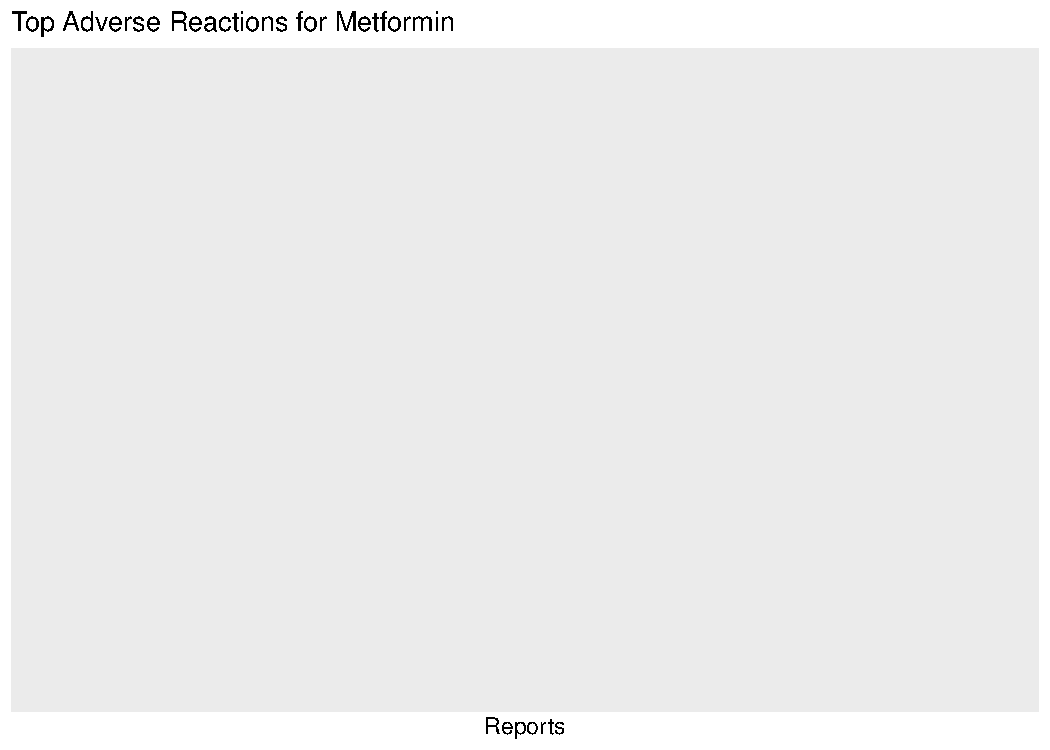
\includegraphics{index_files/figure-pdf/plot-reactions-1.pdf}

\begin{Shaded}
\begin{Highlighting}[]
\NormalTok{ggplot2}\SpecialCharTok{::}\FunctionTok{ggsave}\NormalTok{(}\FunctionTok{glue}\NormalTok{(}\StringTok{"outputs/top\_reactions\_\{drug\}.png"}\NormalTok{), }\AttributeTok{width =} \DecValTok{7}\NormalTok{, }\AttributeTok{height =} \DecValTok{5}\NormalTok{, }\AttributeTok{dpi =} \DecValTok{300}\NormalTok{)}
\end{Highlighting}
\end{Shaded}

\subsubsection{4.3 Age × Sex pattern}\label{age-sex-pattern}

\begin{Shaded}
\begin{Highlighting}[]
\NormalTok{age\_sex }\OtherTok{\textless{}{-}}\NormalTok{ events\_final }\SpecialCharTok{|\textgreater{}}
\NormalTok{  dplyr}\SpecialCharTok{::}\FunctionTok{filter}\NormalTok{(}\SpecialCharTok{!}\FunctionTok{is.na}\NormalTok{(age\_group), sex }\SpecialCharTok{\%in\%} \FunctionTok{c}\NormalTok{(}\StringTok{"Male"}\NormalTok{,}\StringTok{"Female"}\NormalTok{)) }\SpecialCharTok{|\textgreater{}}
\NormalTok{  dplyr}\SpecialCharTok{::}\FunctionTok{count}\NormalTok{(age\_group, sex, }\AttributeTok{sort =} \ConstantTok{TRUE}\NormalTok{) }\SpecialCharTok{|\textgreater{}}
\NormalTok{  dplyr}\SpecialCharTok{::}\FunctionTok{group\_by}\NormalTok{(sex) }\SpecialCharTok{|\textgreater{}}
\NormalTok{  dplyr}\SpecialCharTok{::}\FunctionTok{mutate}\NormalTok{(}\AttributeTok{pct =}\NormalTok{ n }\SpecialCharTok{/} \FunctionTok{sum}\NormalTok{(n)) }\SpecialCharTok{|\textgreater{}}
\NormalTok{  dplyr}\SpecialCharTok{::}\FunctionTok{ungroup}\NormalTok{()}

\NormalTok{knitr}\SpecialCharTok{::}\FunctionTok{kable}\NormalTok{(age\_sex)}
\end{Highlighting}
\end{Shaded}

\begin{longtable}[]{@{}llrr@{}}
\toprule\noalign{}
age\_group & sex & n & pct \\
\midrule\noalign{}
\endhead
\bottomrule\noalign{}
\endlastfoot
\end{longtable}

\begin{Shaded}
\begin{Highlighting}[]
\NormalTok{age\_sex }\SpecialCharTok{\%\textgreater{}\%}
\NormalTok{  ggplot2}\SpecialCharTok{::}\FunctionTok{ggplot}\NormalTok{(ggplot2}\SpecialCharTok{::}\FunctionTok{aes}\NormalTok{(age\_group, n, }\AttributeTok{fill =}\NormalTok{ sex)) }\SpecialCharTok{+}
\NormalTok{  ggplot2}\SpecialCharTok{::}\FunctionTok{geom\_col}\NormalTok{(}\AttributeTok{position =} \StringTok{"dodge"}\NormalTok{) }\SpecialCharTok{+}
\NormalTok{  ggplot2}\SpecialCharTok{::}\FunctionTok{labs}\NormalTok{(}\AttributeTok{title =} \FunctionTok{glue}\NormalTok{(}\StringTok{"\{stringr::str\_to\_title(drug)\}: Reports by Age Group and Sex"}\NormalTok{),}
       \AttributeTok{x =} \StringTok{"Age Group"}\NormalTok{, }\AttributeTok{y =} \StringTok{"Reports"}\NormalTok{) }\SpecialCharTok{+}
\NormalTok{  ggplot2}\SpecialCharTok{::}\FunctionTok{guides}\NormalTok{(}\AttributeTok{fill =}\NormalTok{ ggplot2}\SpecialCharTok{::}\FunctionTok{guide\_legend}\NormalTok{(}\AttributeTok{title =} \StringTok{"Sex"}\NormalTok{))}
\end{Highlighting}
\end{Shaded}

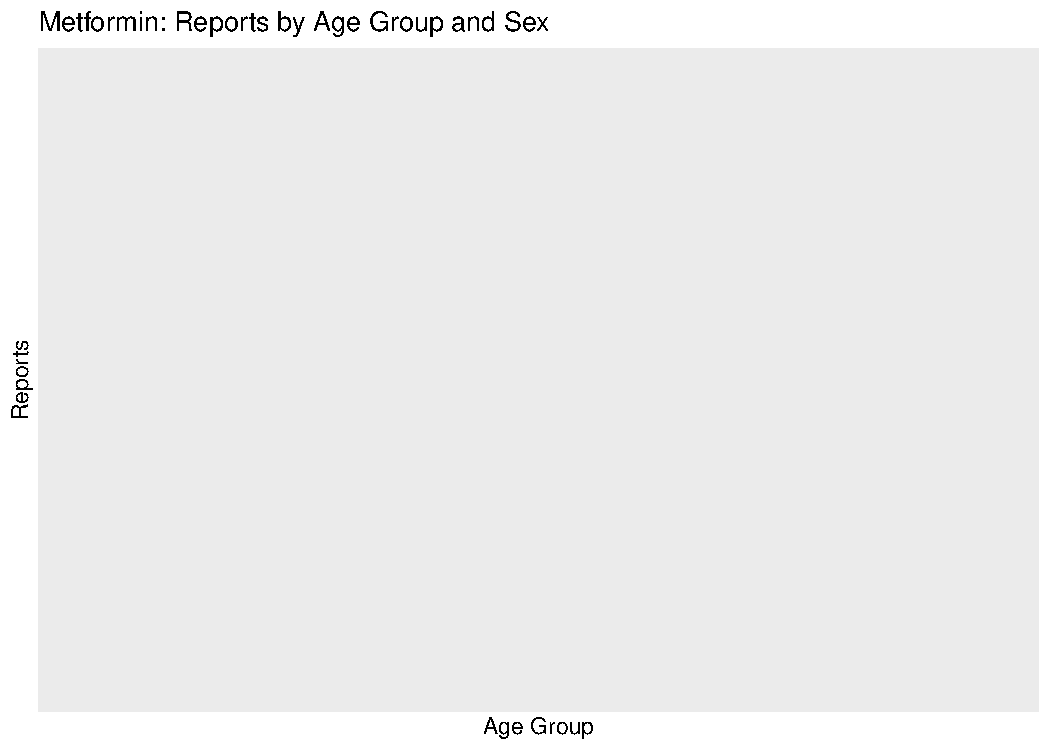
\includegraphics{index_files/figure-pdf/plot-age-sex-1.pdf}

\begin{Shaded}
\begin{Highlighting}[]
\NormalTok{ggplot2}\SpecialCharTok{::}\FunctionTok{ggsave}\NormalTok{(}\FunctionTok{glue}\NormalTok{(}\StringTok{"outputs/age\_sex\_\{drug\}.png"}\NormalTok{), }\AttributeTok{width =} \DecValTok{7}\NormalTok{, }\AttributeTok{height =} \DecValTok{5}\NormalTok{, }\AttributeTok{dpi =} \DecValTok{300}\NormalTok{)}
\end{Highlighting}
\end{Shaded}

\subsubsection{4.4 Serious vs non-serious
outcomes}\label{serious-vs-non-serious-outcomes}

\begin{Shaded}
\begin{Highlighting}[]
\NormalTok{serious\_tbl }\OtherTok{\textless{}{-}}\NormalTok{ events\_final }\SpecialCharTok{|\textgreater{}}
\NormalTok{  dplyr}\SpecialCharTok{::}\FunctionTok{count}\NormalTok{(serious\_flag) }\SpecialCharTok{|\textgreater{}}
\NormalTok{  dplyr}\SpecialCharTok{::}\FunctionTok{mutate}\NormalTok{(}\AttributeTok{pct =}\NormalTok{ scales}\SpecialCharTok{::}\FunctionTok{percent}\NormalTok{(n }\SpecialCharTok{/} \FunctionTok{sum}\NormalTok{(n)))}

\NormalTok{knitr}\SpecialCharTok{::}\FunctionTok{kable}\NormalTok{(serious\_tbl)}
\end{Highlighting}
\end{Shaded}

\begin{longtable}[]{@{}lrl@{}}
\toprule\noalign{}
serious\_flag & n & pct \\
\midrule\noalign{}
\endhead
\bottomrule\noalign{}
\endlastfoot
\end{longtable}

\subsubsection{4.5 Time trend}\label{time-trend}

\begin{Shaded}
\begin{Highlighting}[]
\NormalTok{trend }\OtherTok{\textless{}{-}}\NormalTok{ events\_final }\SpecialCharTok{|\textgreater{}}
\NormalTok{  dplyr}\SpecialCharTok{::}\FunctionTok{mutate}\NormalTok{(}\AttributeTok{month =}\NormalTok{ lubridate}\SpecialCharTok{::}\FunctionTok{floor\_date}\NormalTok{(receivedate, }\StringTok{"month"}\NormalTok{)) }\SpecialCharTok{|\textgreater{}}
\NormalTok{  dplyr}\SpecialCharTok{::}\FunctionTok{count}\NormalTok{(month, }\AttributeTok{name =} \StringTok{"reports"}\NormalTok{)}

\NormalTok{knitr}\SpecialCharTok{::}\FunctionTok{kable}\NormalTok{(}\FunctionTok{head}\NormalTok{(trend, }\DecValTok{12}\NormalTok{))}
\end{Highlighting}
\end{Shaded}

\begin{longtable}[]{@{}lr@{}}
\toprule\noalign{}
month & reports \\
\midrule\noalign{}
\endhead
\bottomrule\noalign{}
\endlastfoot
\end{longtable}

\begin{Shaded}
\begin{Highlighting}[]
\NormalTok{trend }\SpecialCharTok{\%\textgreater{}\%}
\NormalTok{  ggplot2}\SpecialCharTok{::}\FunctionTok{ggplot}\NormalTok{(ggplot2}\SpecialCharTok{::}\FunctionTok{aes}\NormalTok{(month, reports)) }\SpecialCharTok{+}
\NormalTok{  ggplot2}\SpecialCharTok{::}\FunctionTok{geom\_line}\NormalTok{() }\SpecialCharTok{+}
\NormalTok{  ggplot2}\SpecialCharTok{::}\FunctionTok{scale\_y\_continuous}\NormalTok{(}\AttributeTok{labels =}\NormalTok{ scales}\SpecialCharTok{::}\NormalTok{comma) }\SpecialCharTok{+}
\NormalTok{  ggplot2}\SpecialCharTok{::}\FunctionTok{labs}\NormalTok{(}\AttributeTok{title =} \FunctionTok{glue}\NormalTok{(}\StringTok{"\{stringr::str\_to\_title(drug)\}: Monthly Adverse Event Reports"}\NormalTok{),}
       \AttributeTok{x =} \ConstantTok{NULL}\NormalTok{, }\AttributeTok{y =} \StringTok{"Reports"}\NormalTok{)}
\end{Highlighting}
\end{Shaded}

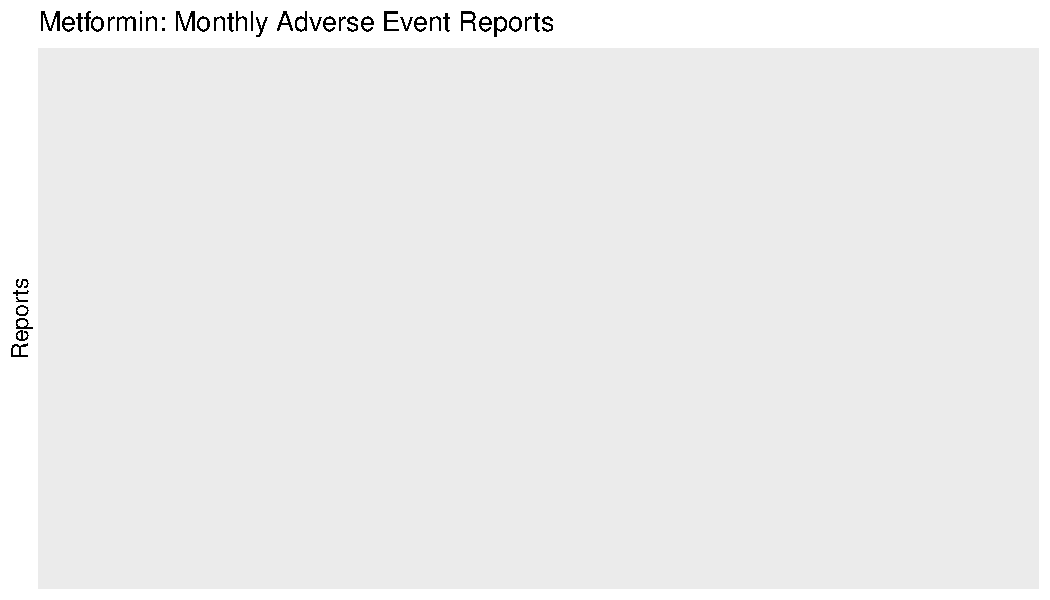
\includegraphics{index_files/figure-pdf/plot-trend-1.pdf}

\begin{Shaded}
\begin{Highlighting}[]
\NormalTok{ggplot2}\SpecialCharTok{::}\FunctionTok{ggsave}\NormalTok{(}\FunctionTok{glue}\NormalTok{(}\StringTok{"outputs/trend\_\{drug\}.png"}\NormalTok{), }\AttributeTok{width =} \DecValTok{7}\NormalTok{, }\AttributeTok{height =} \DecValTok{4}\NormalTok{, }\AttributeTok{dpi =} \DecValTok{300}\NormalTok{)}
\end{Highlighting}
\end{Shaded}

\begin{center}\rule{0.5\linewidth}{0.5pt}\end{center}

\subsection{5. Advisor-Style Summary \&
Recommendations}\label{advisor-style-summary-recommendations}

\begin{Shaded}
\begin{Highlighting}[]
\NormalTok{top3 }\OtherTok{\textless{}{-}}\NormalTok{ top\_rx }\SpecialCharTok{|\textgreater{}}\NormalTok{ dplyr}\SpecialCharTok{::}\FunctionTok{slice\_head}\NormalTok{(}\AttributeTok{n =} \DecValTok{3}\NormalTok{) }\SpecialCharTok{|\textgreater{}}\NormalTok{ dplyr}\SpecialCharTok{::}\FunctionTok{pull}\NormalTok{(reaction) }\SpecialCharTok{|\textgreater{}}\NormalTok{ stringr}\SpecialCharTok{::}\FunctionTok{str\_to\_title}\NormalTok{() }\SpecialCharTok{|\textgreater{}} \FunctionTok{paste}\NormalTok{(}\AttributeTok{collapse =} \StringTok{", "}\NormalTok{)}
\NormalTok{peak\_month }\OtherTok{\textless{}{-}}\NormalTok{ trend }\SpecialCharTok{|\textgreater{}}\NormalTok{ dplyr}\SpecialCharTok{::}\FunctionTok{slice\_max}\NormalTok{(reports, }\AttributeTok{n =} \DecValTok{1}\NormalTok{) }\SpecialCharTok{|\textgreater{}}\NormalTok{ dplyr}\SpecialCharTok{::}\FunctionTok{pull}\NormalTok{(month)}

\NormalTok{summary\_txt }\OtherTok{\textless{}{-}}\NormalTok{ glue}\SpecialCharTok{::}\FunctionTok{glue}\NormalTok{(}\StringTok{"}
\StringTok{**Key Findings (Drug:** \{stringr::str\_to\_title(drug)\} **; Window:** \{start\_date\} → \{end\_date\}**)**  }
\StringTok{• **Top reactions:** \{top3\}.  }
\StringTok{• **Serious outcomes:** \{serious\_tbl |\textgreater{} dplyr::filter(serious\_flag==\textquotesingle{}Serious\textquotesingle{}) |\textgreater{} dplyr::pull(pct)\} of reports marked serious.  }
\StringTok{• **Demographics:** See age×sex chart; consider targeted member education if skewed.  }
\StringTok{• **Utilization trend:** Peak reporting month \textasciitilde{} \{format(peak\_month, \textquotesingle{}\%Y{-}\%m\textquotesingle{})\}.}
\StringTok{"}\NormalTok{)}

\FunctionTok{cat}\NormalTok{(summary\_txt)}
\FunctionTok{writeLines}\NormalTok{(summary\_txt, }\FunctionTok{glue}\NormalTok{(}\StringTok{"outputs/summary\_\{drug\}.md"}\NormalTok{))}
\end{Highlighting}
\end{Shaded}

\subsection{6. Next Steps}\label{next-steps}

\begin{enumerate}
\def\labelenumi{\arabic{enumi}.}
\tightlist
\item
  Increase \texttt{MAX\_PULL\_CAP} to pull more data once you're
  satisfied with speed.\\
\item
  Add \textbf{PRR/ROR disproportionality} for signal detection.\\
\item
  Turn this into a small Quarto site comparing multiple drugs via
  parameters.
\end{enumerate}




\end{document}
